%!TEX TS-program = xelatex
 
% Этот шаблон документа разработан в 2014 году
% Данилом Фёдоровых (danil@fedorovykh.ru) 
% для использования в курсе 
% <<Документы и презентации в \LaTeX>>, записанном НИУ ВШЭ
% для Coursera.org: http://coursera.org/course/latex .
% Исходная версия шаблона --- 
% https://www.writelatex.com/coursera/latex/5.2.2
 
\documentclass[a4paper,12pt]{article}
 
%%% Работа с русским языком
\usepackage[english,russian]{babel}   %% загружает пакет многоязыковой вёрстки
\usepackage{fontspec}      %% подготавливает загрузку шрифтов Open Type, True Type и др.
\defaultfontfeatures{Ligatures={TeX},Renderer=Basic}  %% свойства шрифтов по умолчанию
\setmainfont[Ligatures={TeX,Historic}]{Times New Roman} %% задаёт основной шрифт документа
\setsansfont{Comic Sans MS}                    %% задаёт шрифт без засечек
\setmonofont{Courier New}
\usepackage{indentfirst}
\frenchspacing
 
\renewcommand{\epsilon}{\ensuremath{\varepsilon}}
\renewcommand{\phi}{\ensuremath{\varphi}}
\renewcommand{\kappa}{\ensuremath{\varkappa}}
\renewcommand{\le}{\ensuremath{\leqslant}}
\renewcommand{\leq}{\ensuremath{\leqslant}}
\renewcommand{\ge}{\ensuremath{\geqslant}}
\renewcommand{\geq}{\ensuremath{\geqslant}}
\renewcommand{\emptyset}{\varnothing}
 
%%% Дополнительная работа с математикой
\usepackage{amsmath,amsfonts,amssymb,amsthm,mathtools} % AMS
\usepackage{icomma} % "Умная" запятая: $0,2$ --- число, $0, 2$ --- перечисление
 
%% Номера формул
%\mathtoolsset{showonlyrefs=true} % Показывать номера только у тех формул, на которые есть \eqref{} в тексте.
%\usepackage{leqno} % Нумерация формул слева
 
%% Свои команды
\DeclareMathOperator{\sgn}{\mathop{sgn}}
 
%% Перенос знаков в формулах (по Львовскому)
\newcommand*{\hm}[1]{#1\nobreak\discretionary{}
{\hbox{$\mathsurround=0pt #1$}}{}}
 
%%% Работа с картинками
\usepackage{graphicx}  % Для вставки рисунков
\graphicspath{{images/}{images2/}}  % папки с картинками
\setlength\fboxsep{3pt} % Отступ рамки \fbox{} от рисунка
\setlength\fboxrule{1pt} % Толщина линий рамки \fbox{}
\usepackage{wrapfig} % Обтекание рисунков текстом
 
%%% Работа с таблицами
\usepackage{array,tabularx,tabulary,booktabs} % Дополнительная работа с таблицами
\usepackage{longtable}  % Длинные таблицы
\usepackage{multirow} % Слияние строк в таблице
 
%%% Теоремы
\theoremstyle{plain} % Это стиль по умолчанию, его можно не переопределять.
\newtheorem{theorem}{Теорема}[section]
\newtheorem{proposition}[theorem]{Утверждение}
 
\theoremstyle{definition} % "Определение"
\newtheorem{corollary}{Следствие}[theorem]
\newtheorem{problem}{Задача}[section]
 
\theoremstyle{remark} % "Примечание"
\newtheorem*{nonum}{Решение}
 
%%% Программирование
\usepackage{etoolbox} % логические операторы
 
 
%%% Страница
\usepackage{extsizes} % Возможность сделать 14-й шрифт
\usepackage{geometry} % Простой способ задавать поля
	\geometry{top=5mm}
	\geometry{bottom=15mm}
	\geometry{left=5mm}
	\geometry{right=5mm}
 %
%\usepackage{fancyhdr} % Колонтитулы
% 	\pagestyle{fancy}
 	%\renewcommand{\headrulewidth}{0pt}  % Толщина линейки, отчеркивающей верхний колонтитул
% 	\lfoot{Нижний левый}
% 	\rfoot{Нижний правый}
% 	\rhead{Верхний правый}
% 	\chead{Верхний в центре}
% 	\lhead{Верхний левый}
%	\cfoot{Нижний в центре} % По умолчанию здесь номер страницы
 
\usepackage{setspace} % Интерлиньяж
%\onehalfspacing % Интерлиньяж 1.5
%\doublespacing % Интерлиньяж 2
%\singlespacing % Интерлиньяж 1
 
\usepackage{lastpage} % Узнать, сколько всего страниц в документе.
 
\usepackage{soul} % Модификаторы начертания
 
\usepackage{hyperref}
\usepackage[usenames,dvipsnames,svgnames,table,rgb]{xcolor}
\hypersetup{				% Гиперссылки
    unicode=true,           % русские буквы в раздела PDF
    pdftitle={Заголовок},   % Заголовок
    pdfauthor={Автор},      % Автор
    pdfsubject={Тема},      % Тема
    pdfcreator={Создатель}, % Создатель
    pdfproducer={Производитель}, % Производитель
    pdfkeywords={keyword1} {key2} {key3}, % Ключевые слова
    colorlinks=true,       	% false: ссылки в рамках; true: цветные ссылки
    linkcolor=red,          % внутренние ссылки
    citecolor=black,        % на библиографию
    filecolor=magenta,      % на файлы
    urlcolor=cyan           % на URL
}
 
\usepackage{csquotes} % Еще инструменты для ссылок
 
%\usepackage[style=authoryear,maxcitenames=2,backend=biber,sorting=nty]{biblatex}
 
\usepackage{multicol} % Несколько колонок
 
\usepackage{tikz} % Работа с графикой
\usepackage{pgfplots}
\usepackage{pgfplotstable}
 
\author{Батарин Егор}
\title{Туннелирование в СВЧ диапазоне.}
\date{\today}
 
\begin{document} % конец преамбулы, начало документа
 
\maketitle
 
\begin{abstract}
   Цель работы: исследование эффекта туннелирования радиоволн миллиметрового диапазона, проведение измерений в хеме Майкельсона.
\end{abstract}
 
\section{Теория}

Проникновение электромагнитных волн в менее плотную среду при полном внутреннем отражении - явление той же природы, что и проникновение частиц в область, где их полная энергия оказывается меньше потенциальной энергии. Это явление изучается в квантовой физике и носит название \textbf{туннельного эффекта}. 

\begin{figure}[h!]
	\center{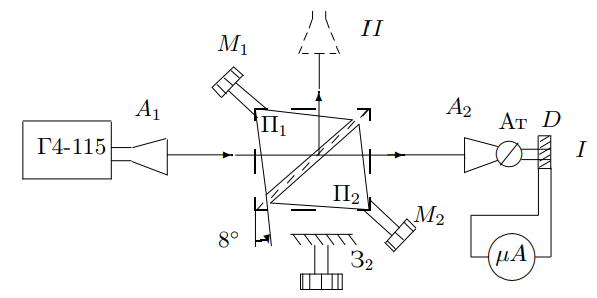
\includegraphics[scale = 0.8]{1.png}}
	\caption{Схема установки}
\end{figure}

Исследуем этот эффект - проникновение ЭМВ через воздушный зазор между диэлектрическими призмами при полном внутреннем отражении на границе диэлектрик-воздух. Моделирование интерферометра Майкельсона с использованием этого эффекта и измерение длины волны излучения и показателя преломления фторопласта для радиоволн миллиметрового диапазона. 

Для измерения показателя преломления матриала призм мы установим пластину толщины $h$ из того же матриала, что и призмы - фторопласта. Имеем тогда приращение длины "оптического пути" \[\Delta{} = 2h(n - 1).\]

Данное приращение можно скомпенсировать, передвинув подвижное зеркало на необходимое расстояние $\delta{}x:$ \[\delta{}x = h(n-1).\]

Для толстых пластин, когда $\Delta > \lambda$, необходимо учесть изменение порядка интерференции. Это можно сделать, зная приближенное значение показателя преломления флоропласта ($n \approx 1.5$)

\section{Выполнение}
\begin{enumerate}
\item Исследование туннелирования СВЧ волн.

Рабочая частота клистрона - от $35.93$ ГГЦ до  $35.99$ ГГц, мы использовали $35.96$ ГГц.Ей соответствует длина волны $\lambda = \frac{c}{\nu} = 8.34 \pm 0.01$ мм. Мощность на 38 Вт. 100 Дел = 10 мкА, значит 1 Дел = 100 нА. Затем мы gереставим приемник для измерения отраженного света. Получится зависимость для преломленного и отраженного света:

\begin{figure}[h!]
	\center{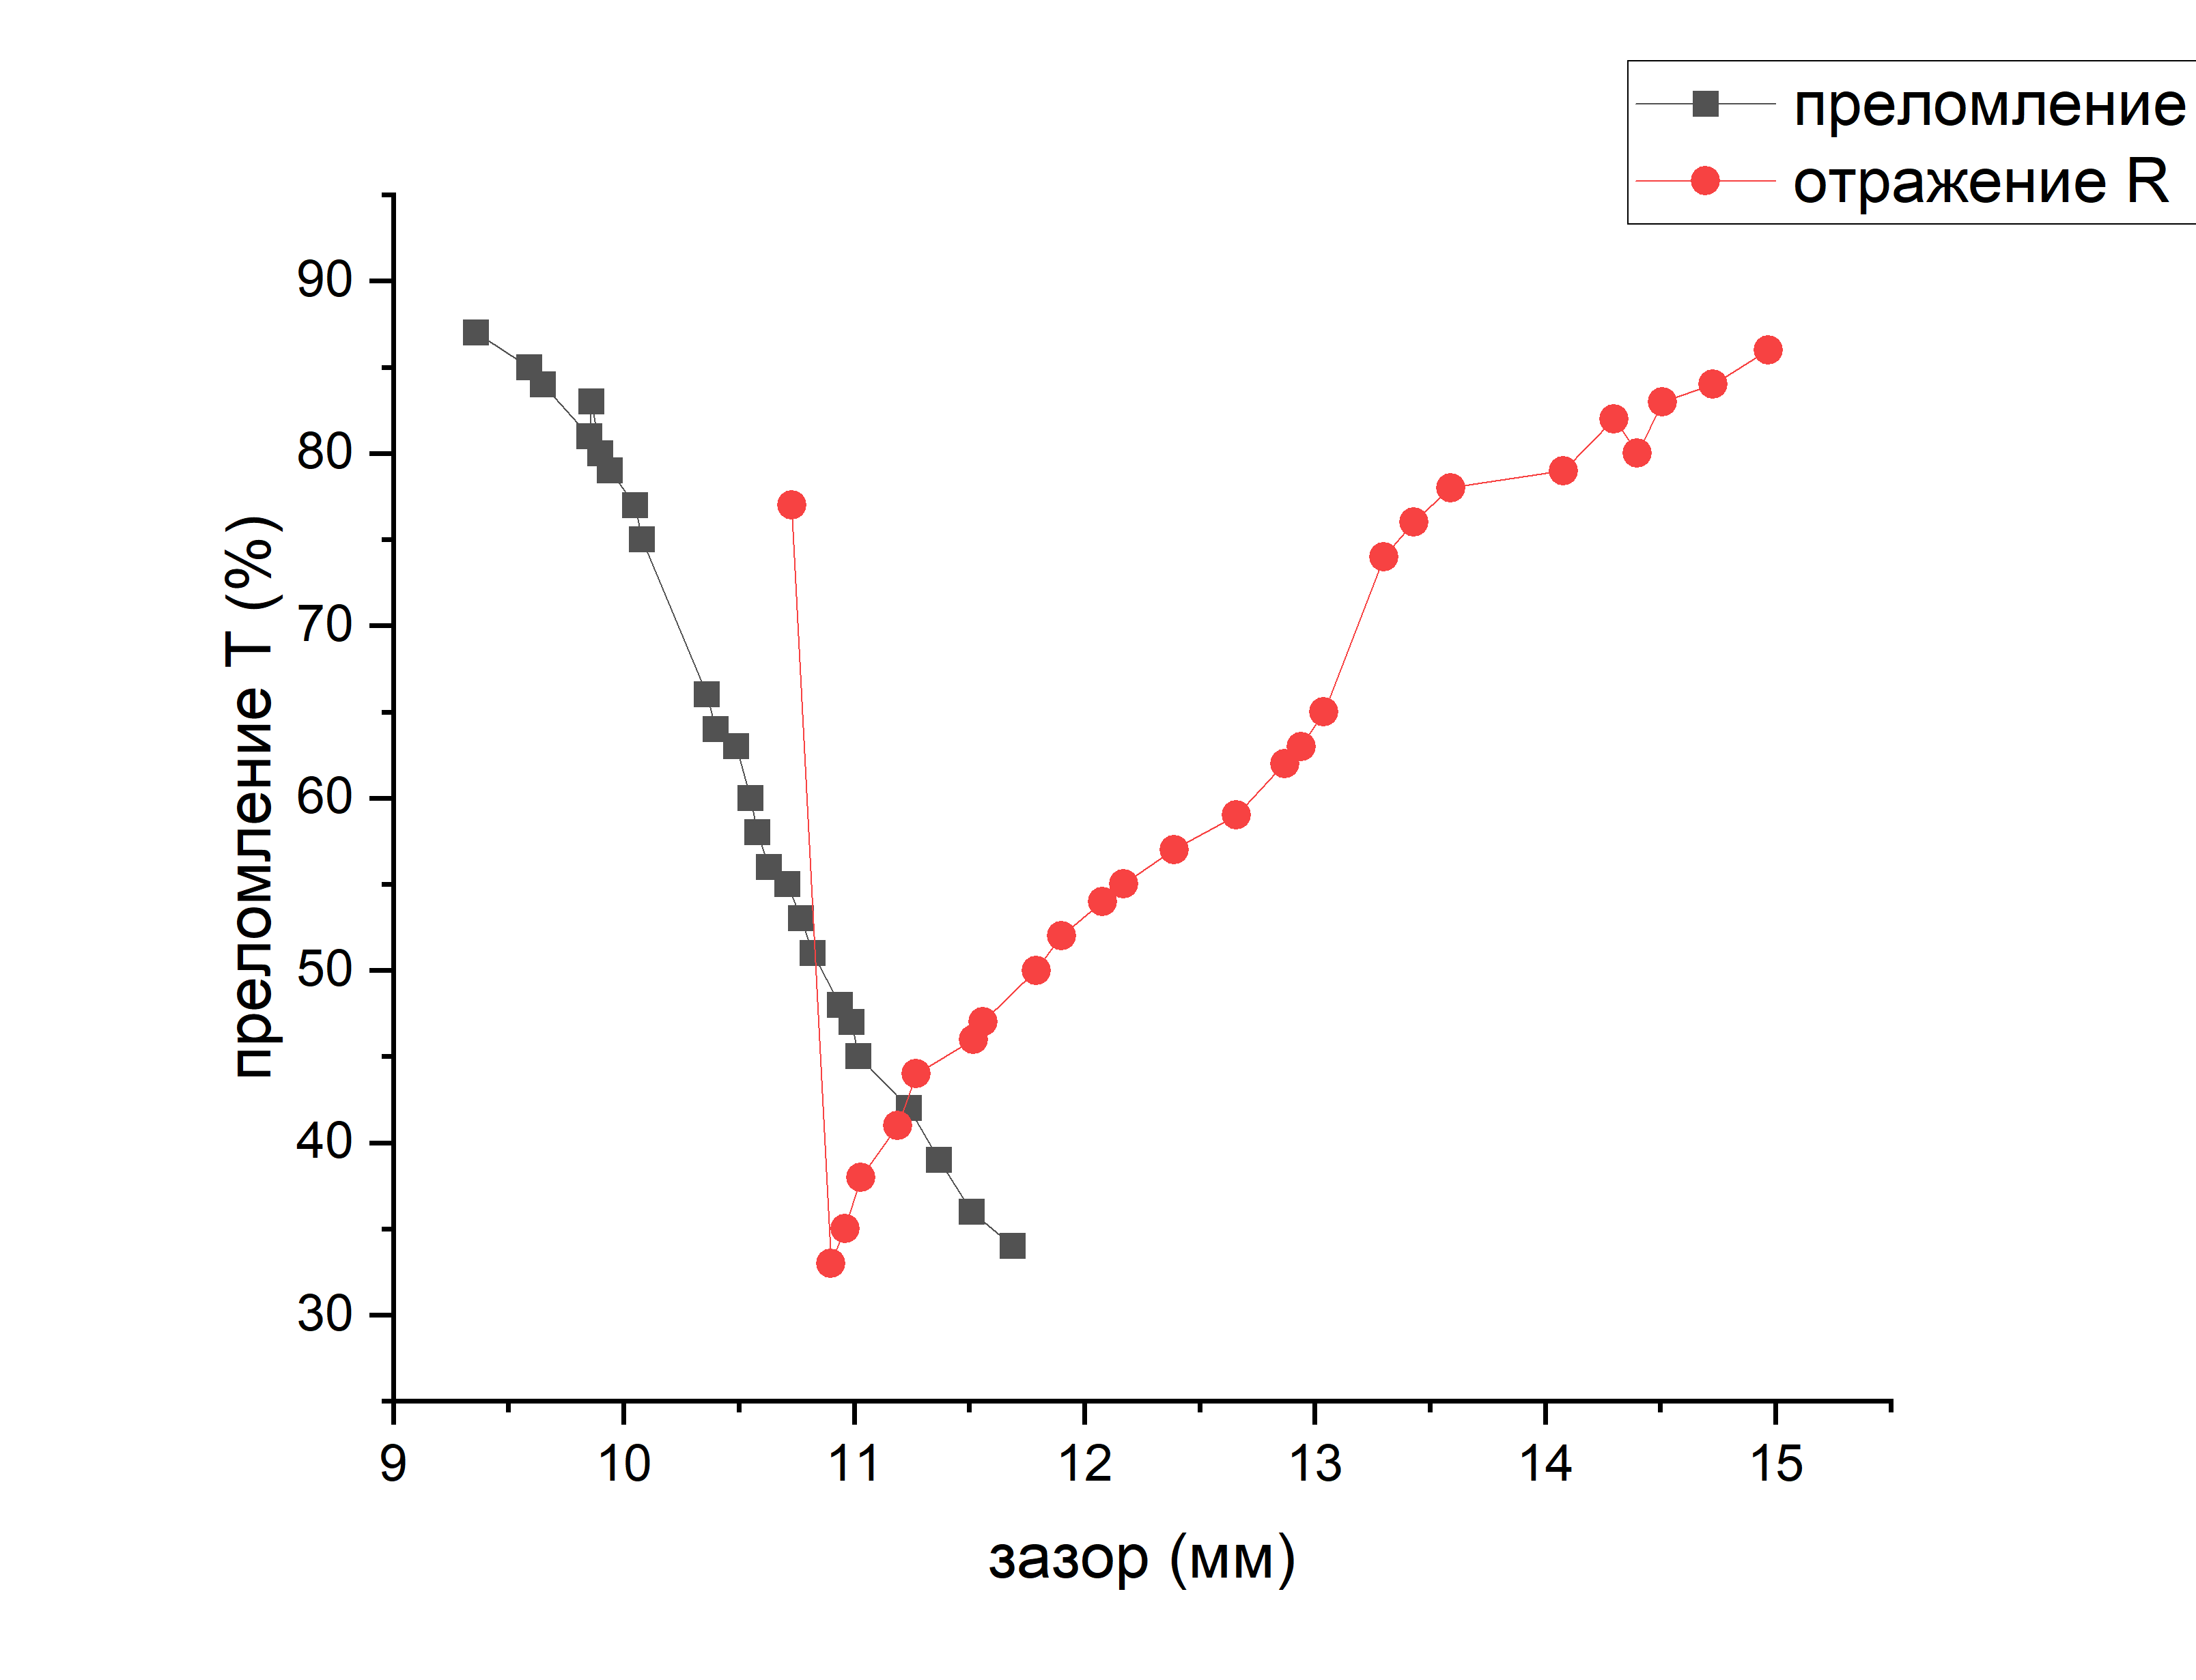
\includegraphics[scale = 0.4]{2.png}}
	\caption{Зависимость $T$ и $R$ от $l$}
\end{figure}

Отсюда видно, что $T+R \approx 1$. Далее строим график $\ln(T) = f(z)$:

\begin{figure}[h!]
	\center{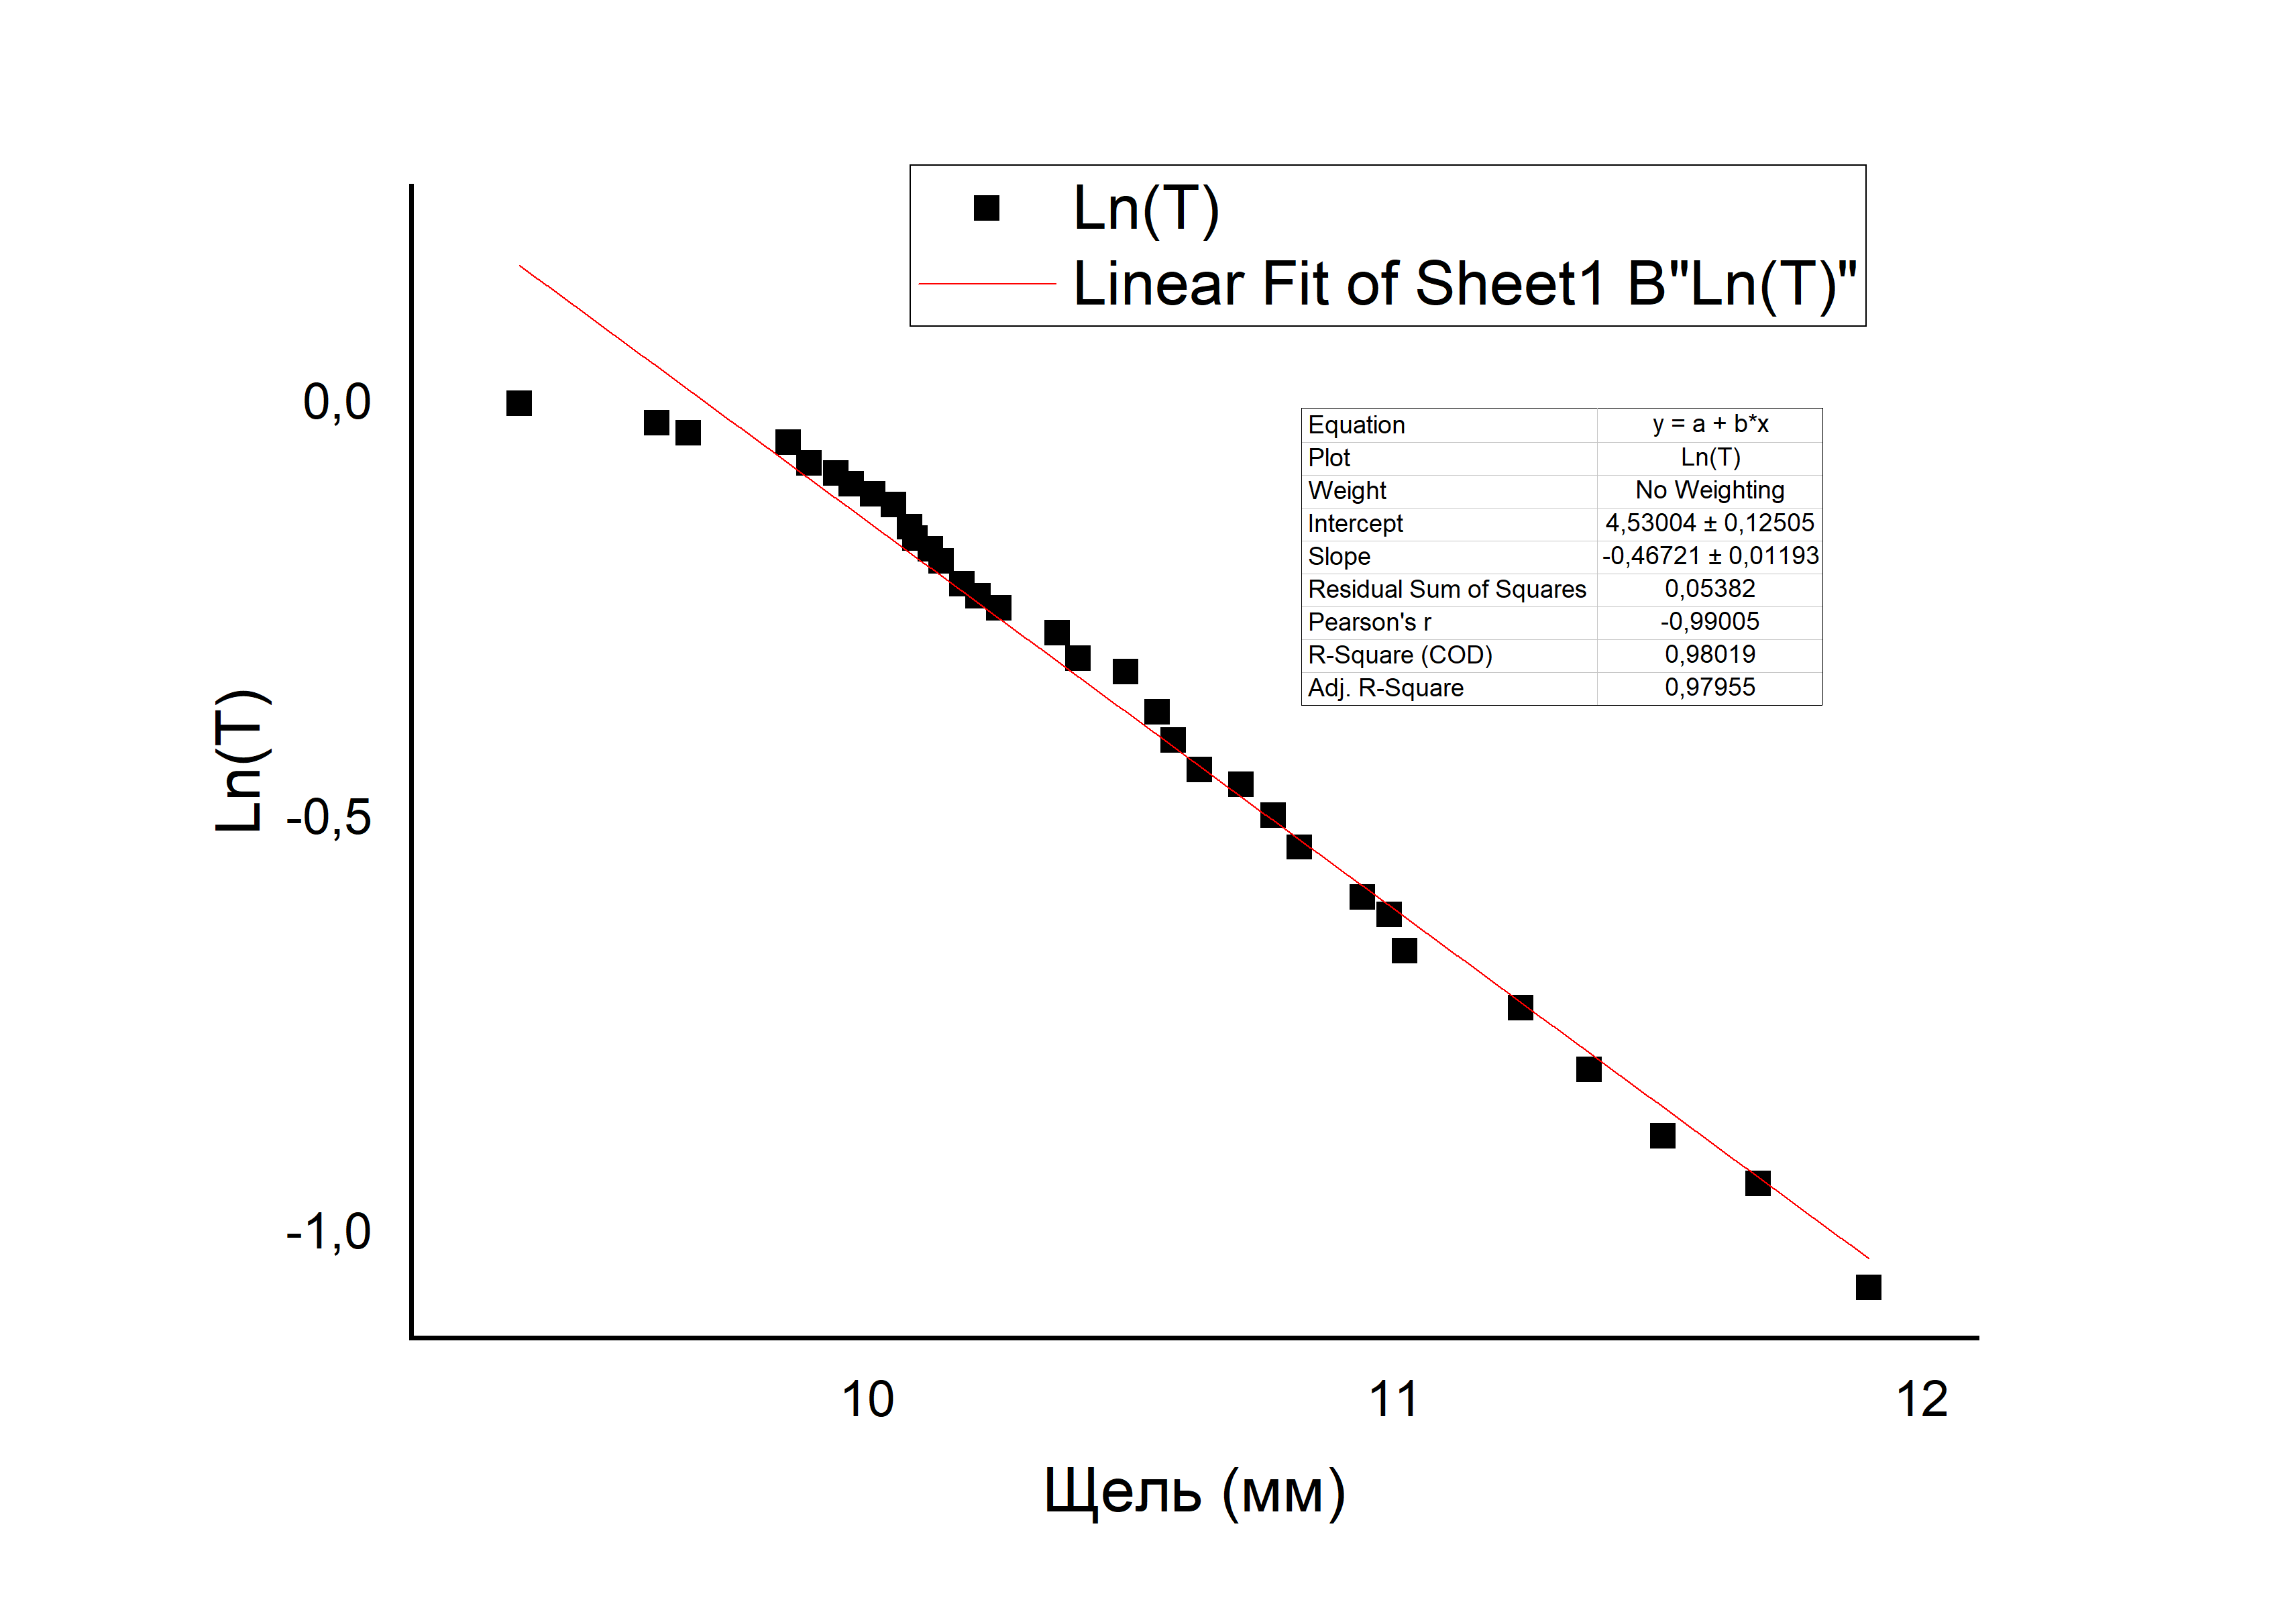
\includegraphics[scale = 0.4]{3.png}}
	\caption{$\ln(T) = f(z)$}
\end{figure}

Далее вычисляем показатель преломления $n$ с учетом того, что $\Lambda = 0.46 \pm 0.01$ и $\phi \approx \frac{\pi}{4}$:
\[
n = \frac{1}{\sin\phi}\sqrt{1+ \frac{1}{(4\pi\Lambda)^2}} = 1.4 \pm 0.1 \text{мм}
\]
Это хорошо соотносится с табличным значением $1.46$.x`
\item Интерферометр Майкельсона

Установим зазор такой, что $T = R \approx 0.5$. Собираем схему Майкельсона. Снимаем зависимость силы тока $I = f(x)$ от координаты $x$ подвижного зеркала. Получаем  зависимость:
\begin{figure}[h!]
	\center{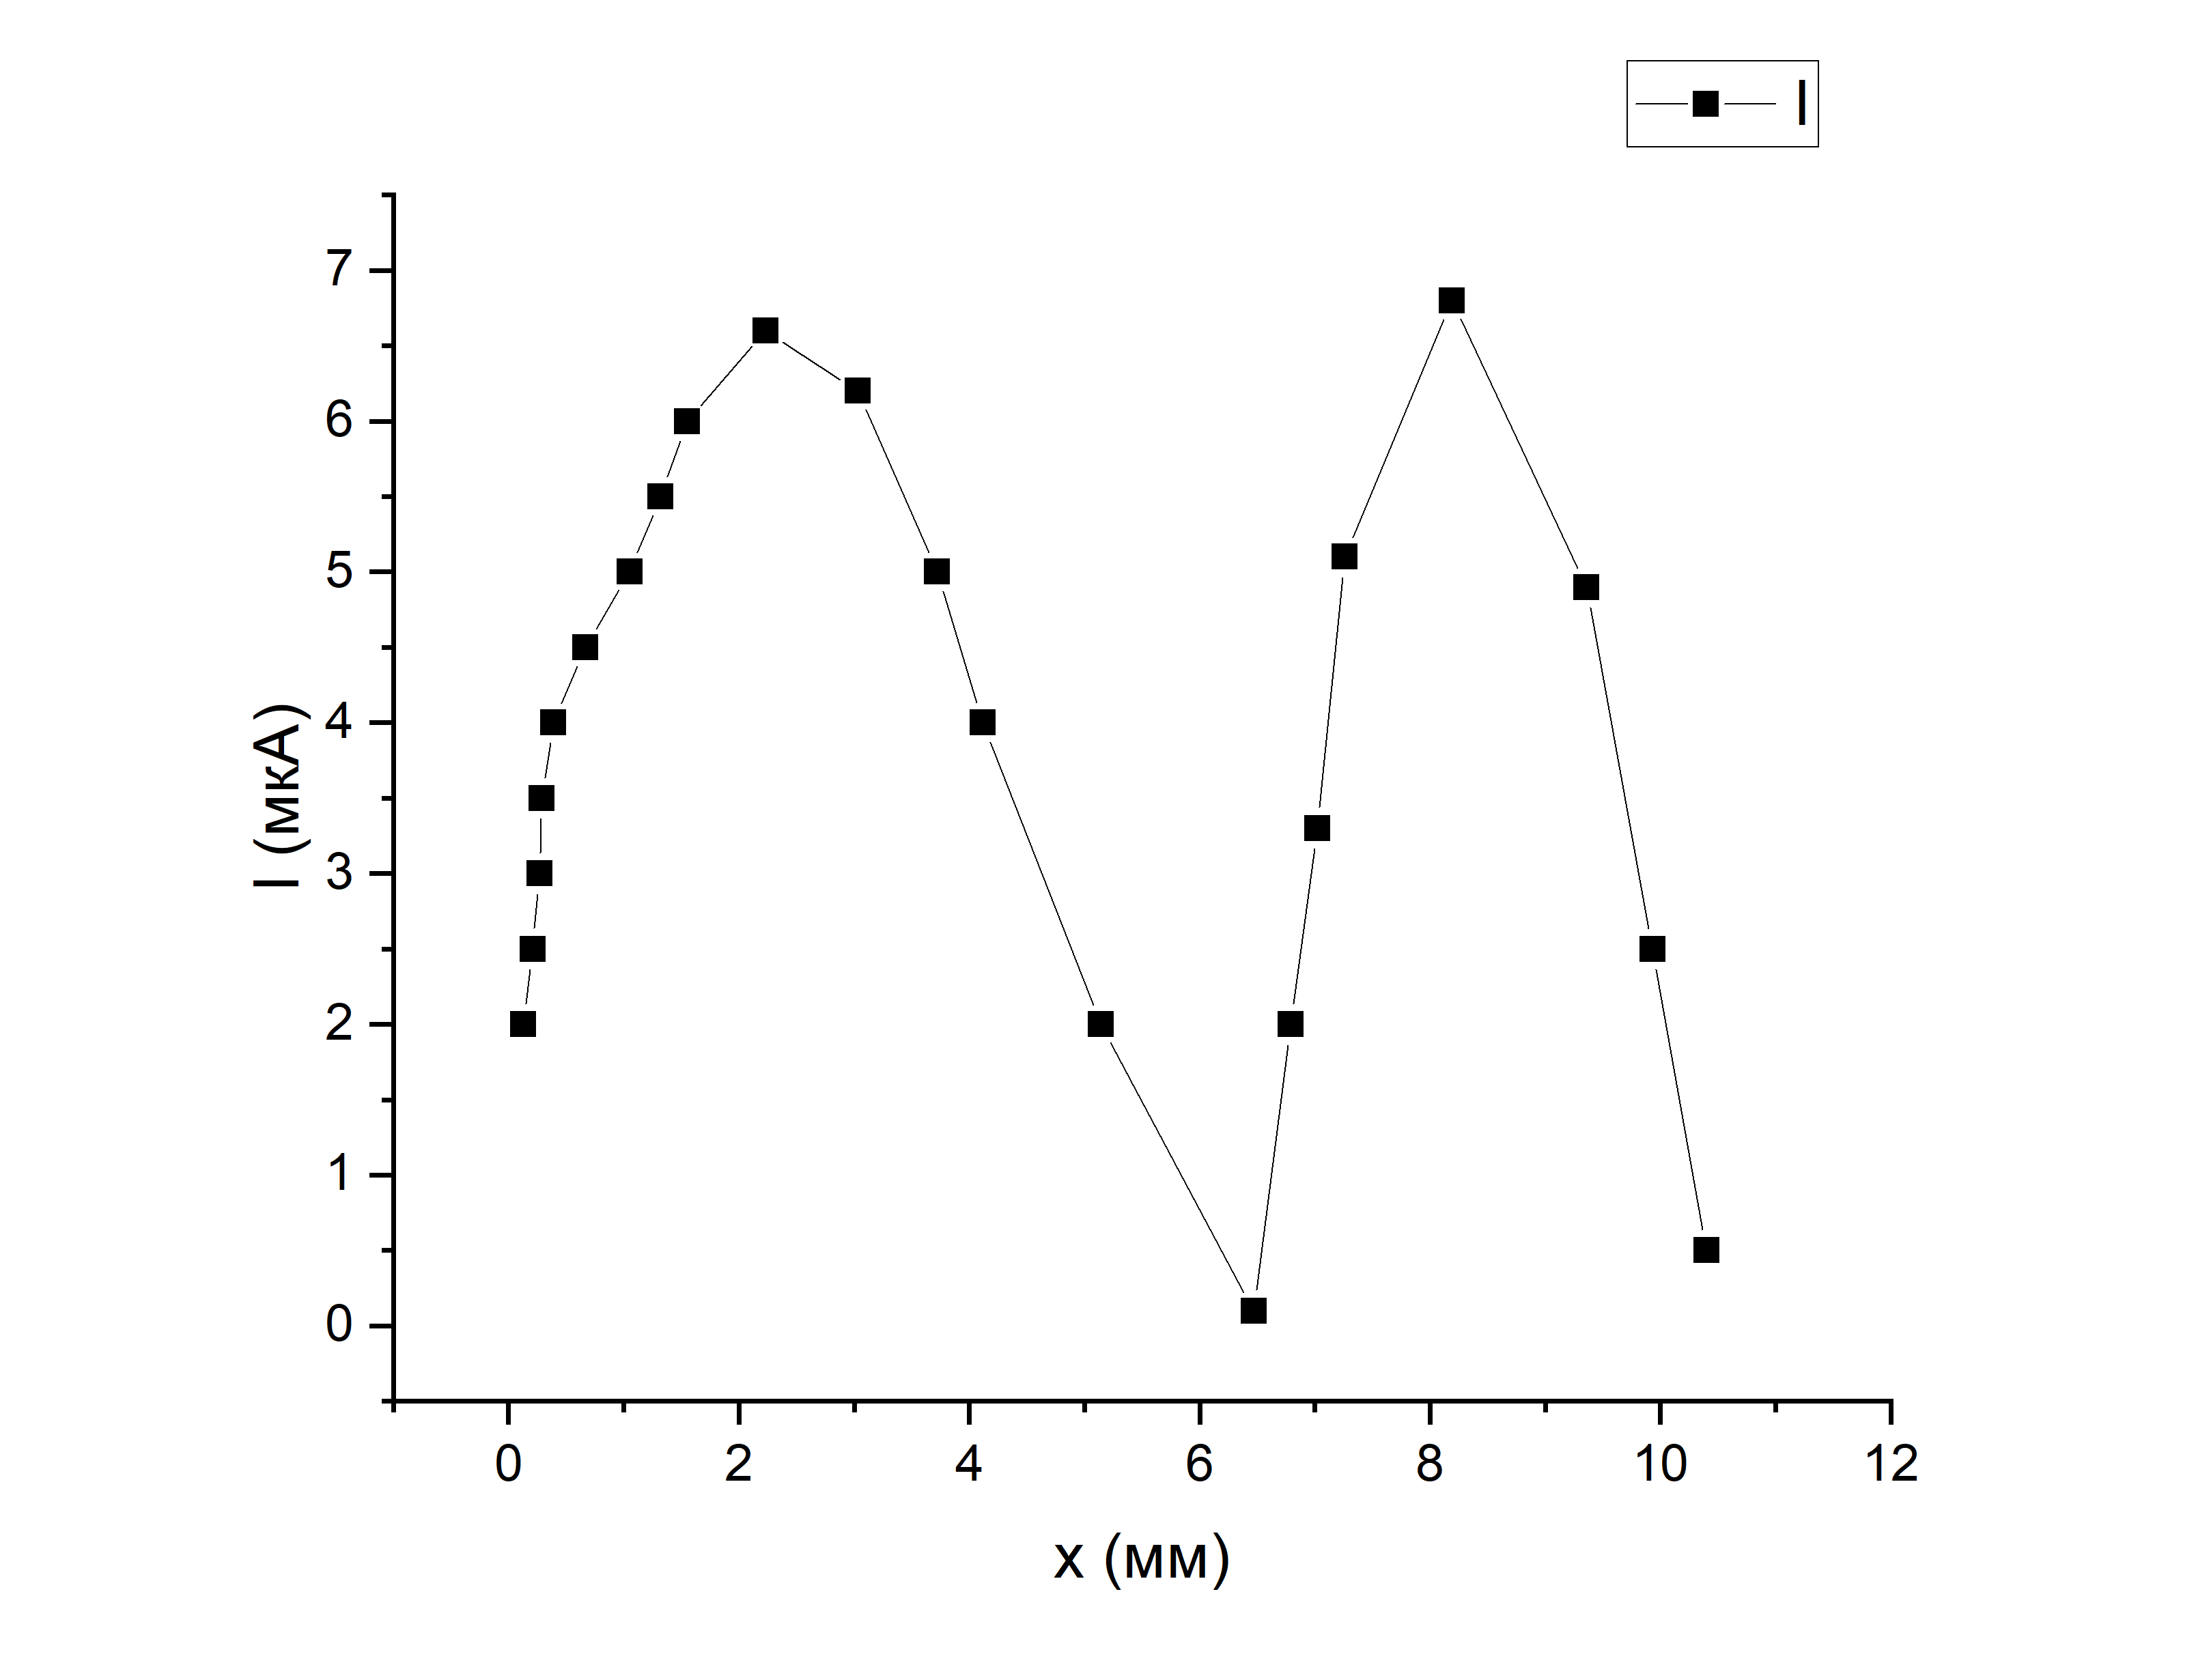
\includegraphics[scale = 0.4]{4.png}}
	\caption{Подвижное зеркало}
\end{figure}
Далее вставим пластину фторопласта с $h \approx 6.2$ мм. Получаем расстояние $\delta x = \frac{1.5+2+1.82}{3} = 1.77  $ мм.
Теперь можно вычислить показатель преломления:
\[
n = 1 + \frac{\delta x }{h} = 1.3 \pm 0.1 \text{мм}
\]
Это уже дальше от правды, но мы старались :-)

\section{Вывод}

В работе получена зависимость $T$ и $R$ от $l$ и $\ln(T) = f(z)$. По первому графику подтвердилось соотношение $T+R \approx 1$, по второму получилось значение $n = 1.4 \pm 0.1$ мм, совпадающее с табличным в пределах погрешностей.
Тем не менее, значение $n = 1.3 \pm 0.1 $ мм, измеренное интерферометром Майкельсона, оказалось далеким от правды.






\end{enumerate}

\end{document} % конец документа